\documentclass[a4,10pt,zihao=-4]{ctexart}
\linespread{1.0} % 设置单倍行距

\usepackage{ctex}
\usepackage[utf8]{inputenc}
\usepackage{amsfonts,amsmath,amscd,amssymb,amsthm}
\usepackage{latexsym,bm}
\usepackage{cite}
\usepackage{mathtools,mathdots,graphicx,array}
\usepackage{fancyhdr}
\usepackage{lastpage}
\usepackage{color}
\usepackage{enumitem}
\usepackage{mpdoc}
\usepackage{diagbox}
\usepackage{xcolor,tcolorbox,tikz,tkz-tab,mdframed,tikz-cd}
\usepackage{framed}
\usepackage{verbatim}
\usepackage{extarrows}
\usepackage{fontspec}
\graphicspath{{./assets/}}  % 设置图片的默认路径

\begin{document}
\pagenumbering{roman}
\title{实验一\,\,\,\,基础电路的实现与测试}

\author{李雨轩 2204112913 计算机2205}
\date{2024年5月}
\maketitle

\section{实验目的}
\begin{enumerate}
  \item 掌握Verilog语言框架,编程及调试的方法。
  \item 熟悉Verilog的基本语法。
  \item 掌握Vivado开发平台及FPGA开发板的使用。
\end{enumerate}

\section{实验内容}
\begin{enumerate}
  \item 利用“Vivado Test”目录下的实例,在Vivado中完成一个工程的设计、编辑、综合和实现的全过程(拍照记录开发板运行结果,简要分析对开发过程和三种文件作用的理解)。
  \item 完成基本电路模块的设计与测试(只执行SIMULATION与RTL ANALYSIS,不用下载到开发板),说明电路功能,分析设计代码实现、RTL电路图、仿真代码及仿真结果。
\end{enumerate}

\section{实验要求}
\begin{enumerate}
  \item 说明电路功能,分析设计、仿真代码和电路图。
  \item 分析仿真波形,观察输入输出是否与预期电路功能相符(测试要全面,关注特殊情况的测试)。
  \item 记录设计和调试过程。
\end{enumerate}

\section{实验过程及结果分析}
\subsection{验证Vivado完整的开发流程}



在本次实验中,我们的主要目的是验证Vivado完整的开发流程,并掌握Vivado平台、Verilog语言和开发板的使用。下面是实验过程:

\begin{enumerate}
\item
  新建工程:首先,我们在Vivado中创建了一个新的RTL工程,命名为RTLProject。在此过程中,我们选择了目标芯片为EGo1开发板:xc7a35tcsg324-1,这是为了确保我们的设计与目标硬件平台相兼容。
\item
  编写/导入文件:在新建工程后,我们导入了实验指导者提供的三个文件,包括源文件、仿真文件和约束文件。这三个文件描述了在EGo1开发板上实现流水灯效果的详细设计。在导入这些文件之前,我们需要理解每个文件的作用,并确保它们之间的关联正确。
\item
  时序仿真、RTL分析:在导入文件后,我们进行了时序仿真和RTL分析。时序仿真能够模拟设计在不同条件下的行为,并产生相应的波形图,从而验证设计的正确性和时序逻辑。RTL分析则可以检查设计的逻辑结构是否与预期一致。
    \begin{itemize}
    \item RTL分析结果:
      
      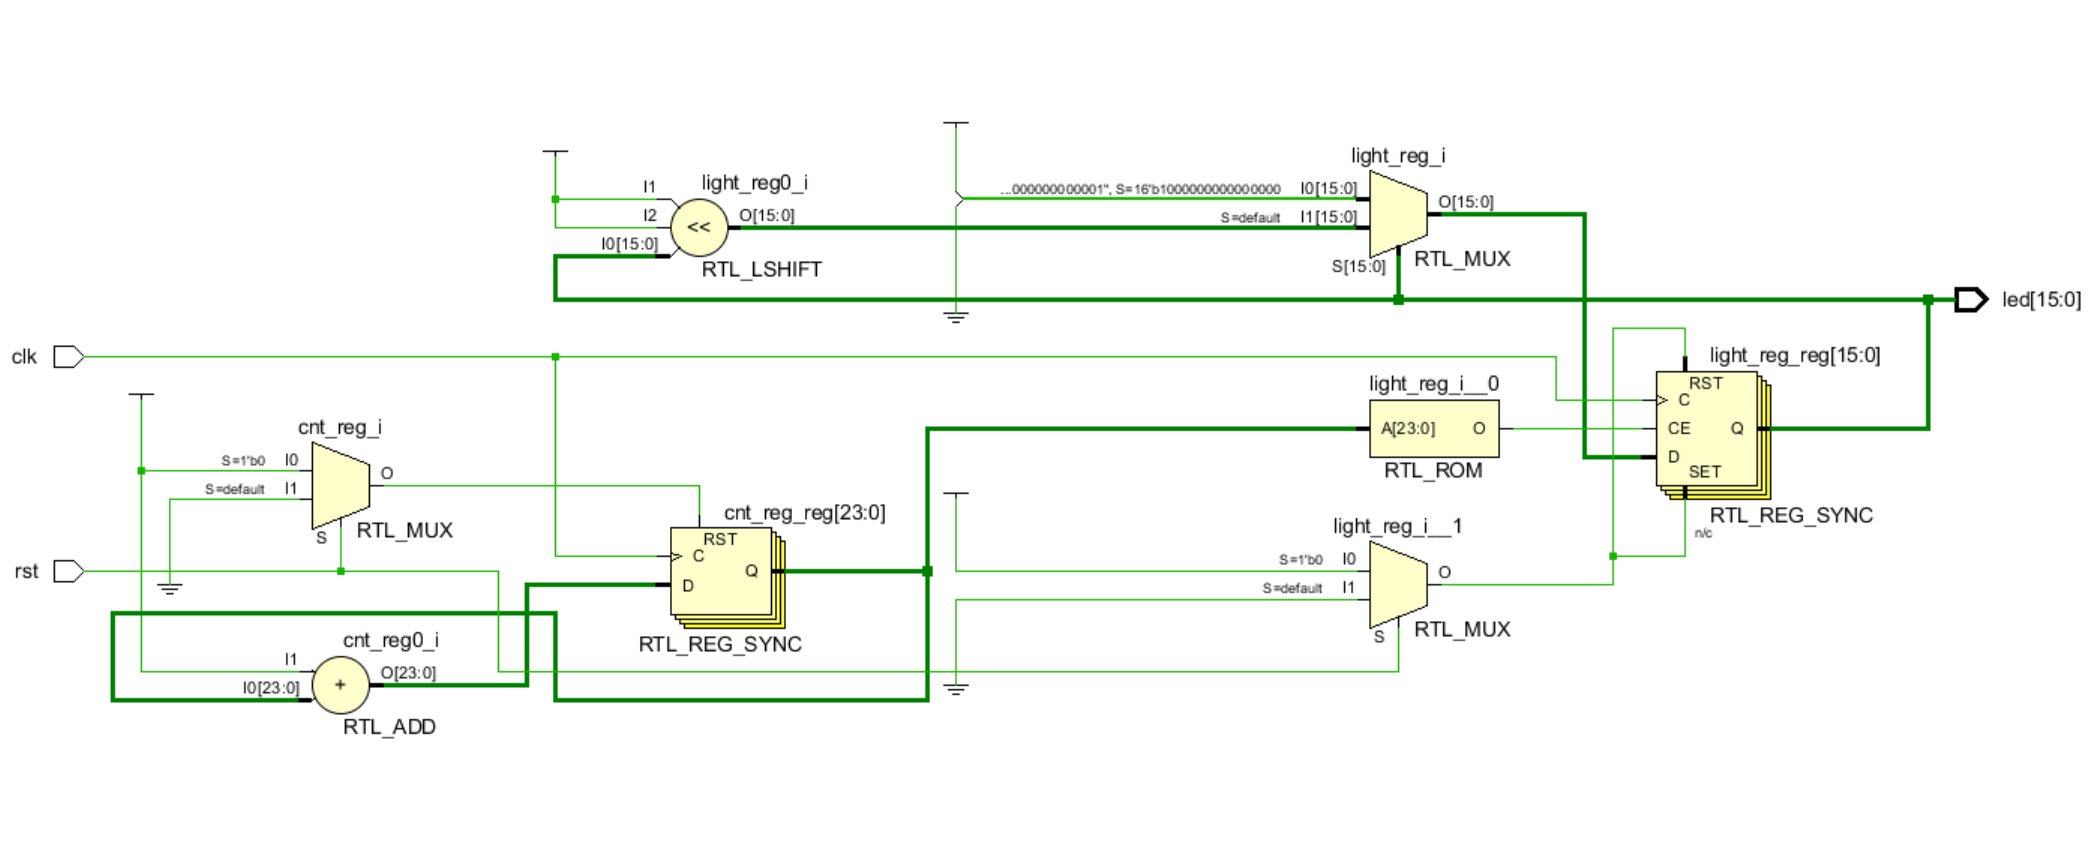
\includegraphics[width=0.5\textwidth]{Flowing_light_RTL.png}
    \item Simulation结果:
      
      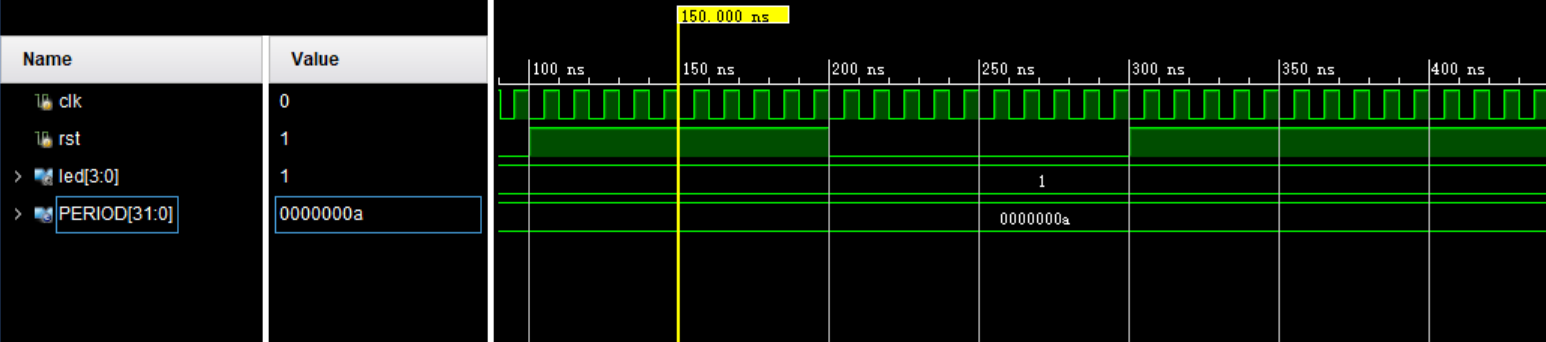
\includegraphics[width=0.5\textwidth]{Flowing_light_Simulation.png}
    \end{itemize}
\item
  约束:在进行约束之前,我们需要了解每个信号在FPGA芯片上的引脚分配情况。通过约束文件,我们可以指定设计中各个信号与FPGA芯片引脚的对应关系,以确保设计在硬件上的正确连接。这一步骤对于设计的成功实现至关重要。
\item
  综合:综合是将Verilog代码转换为逻辑门级的网表的过程。在综合过程中,Vivado会进行逻辑综合和优化,生成适合FPGA实现的网表。我们需要确保综合后的设计逻辑满足预期,并且能够在目标芯片上实现。
\item
  生成二进制文件,下载到板卡验证:最后,我们生成了二进制文件,并下载到FPGA开发板上进行验证。通过验证,我们确认了设计在实际硬件上的运行情况,并成功实现了流水灯(Flowing\_Light)效果:开发板内部时钟驱动的LED灯流水亮灭。

  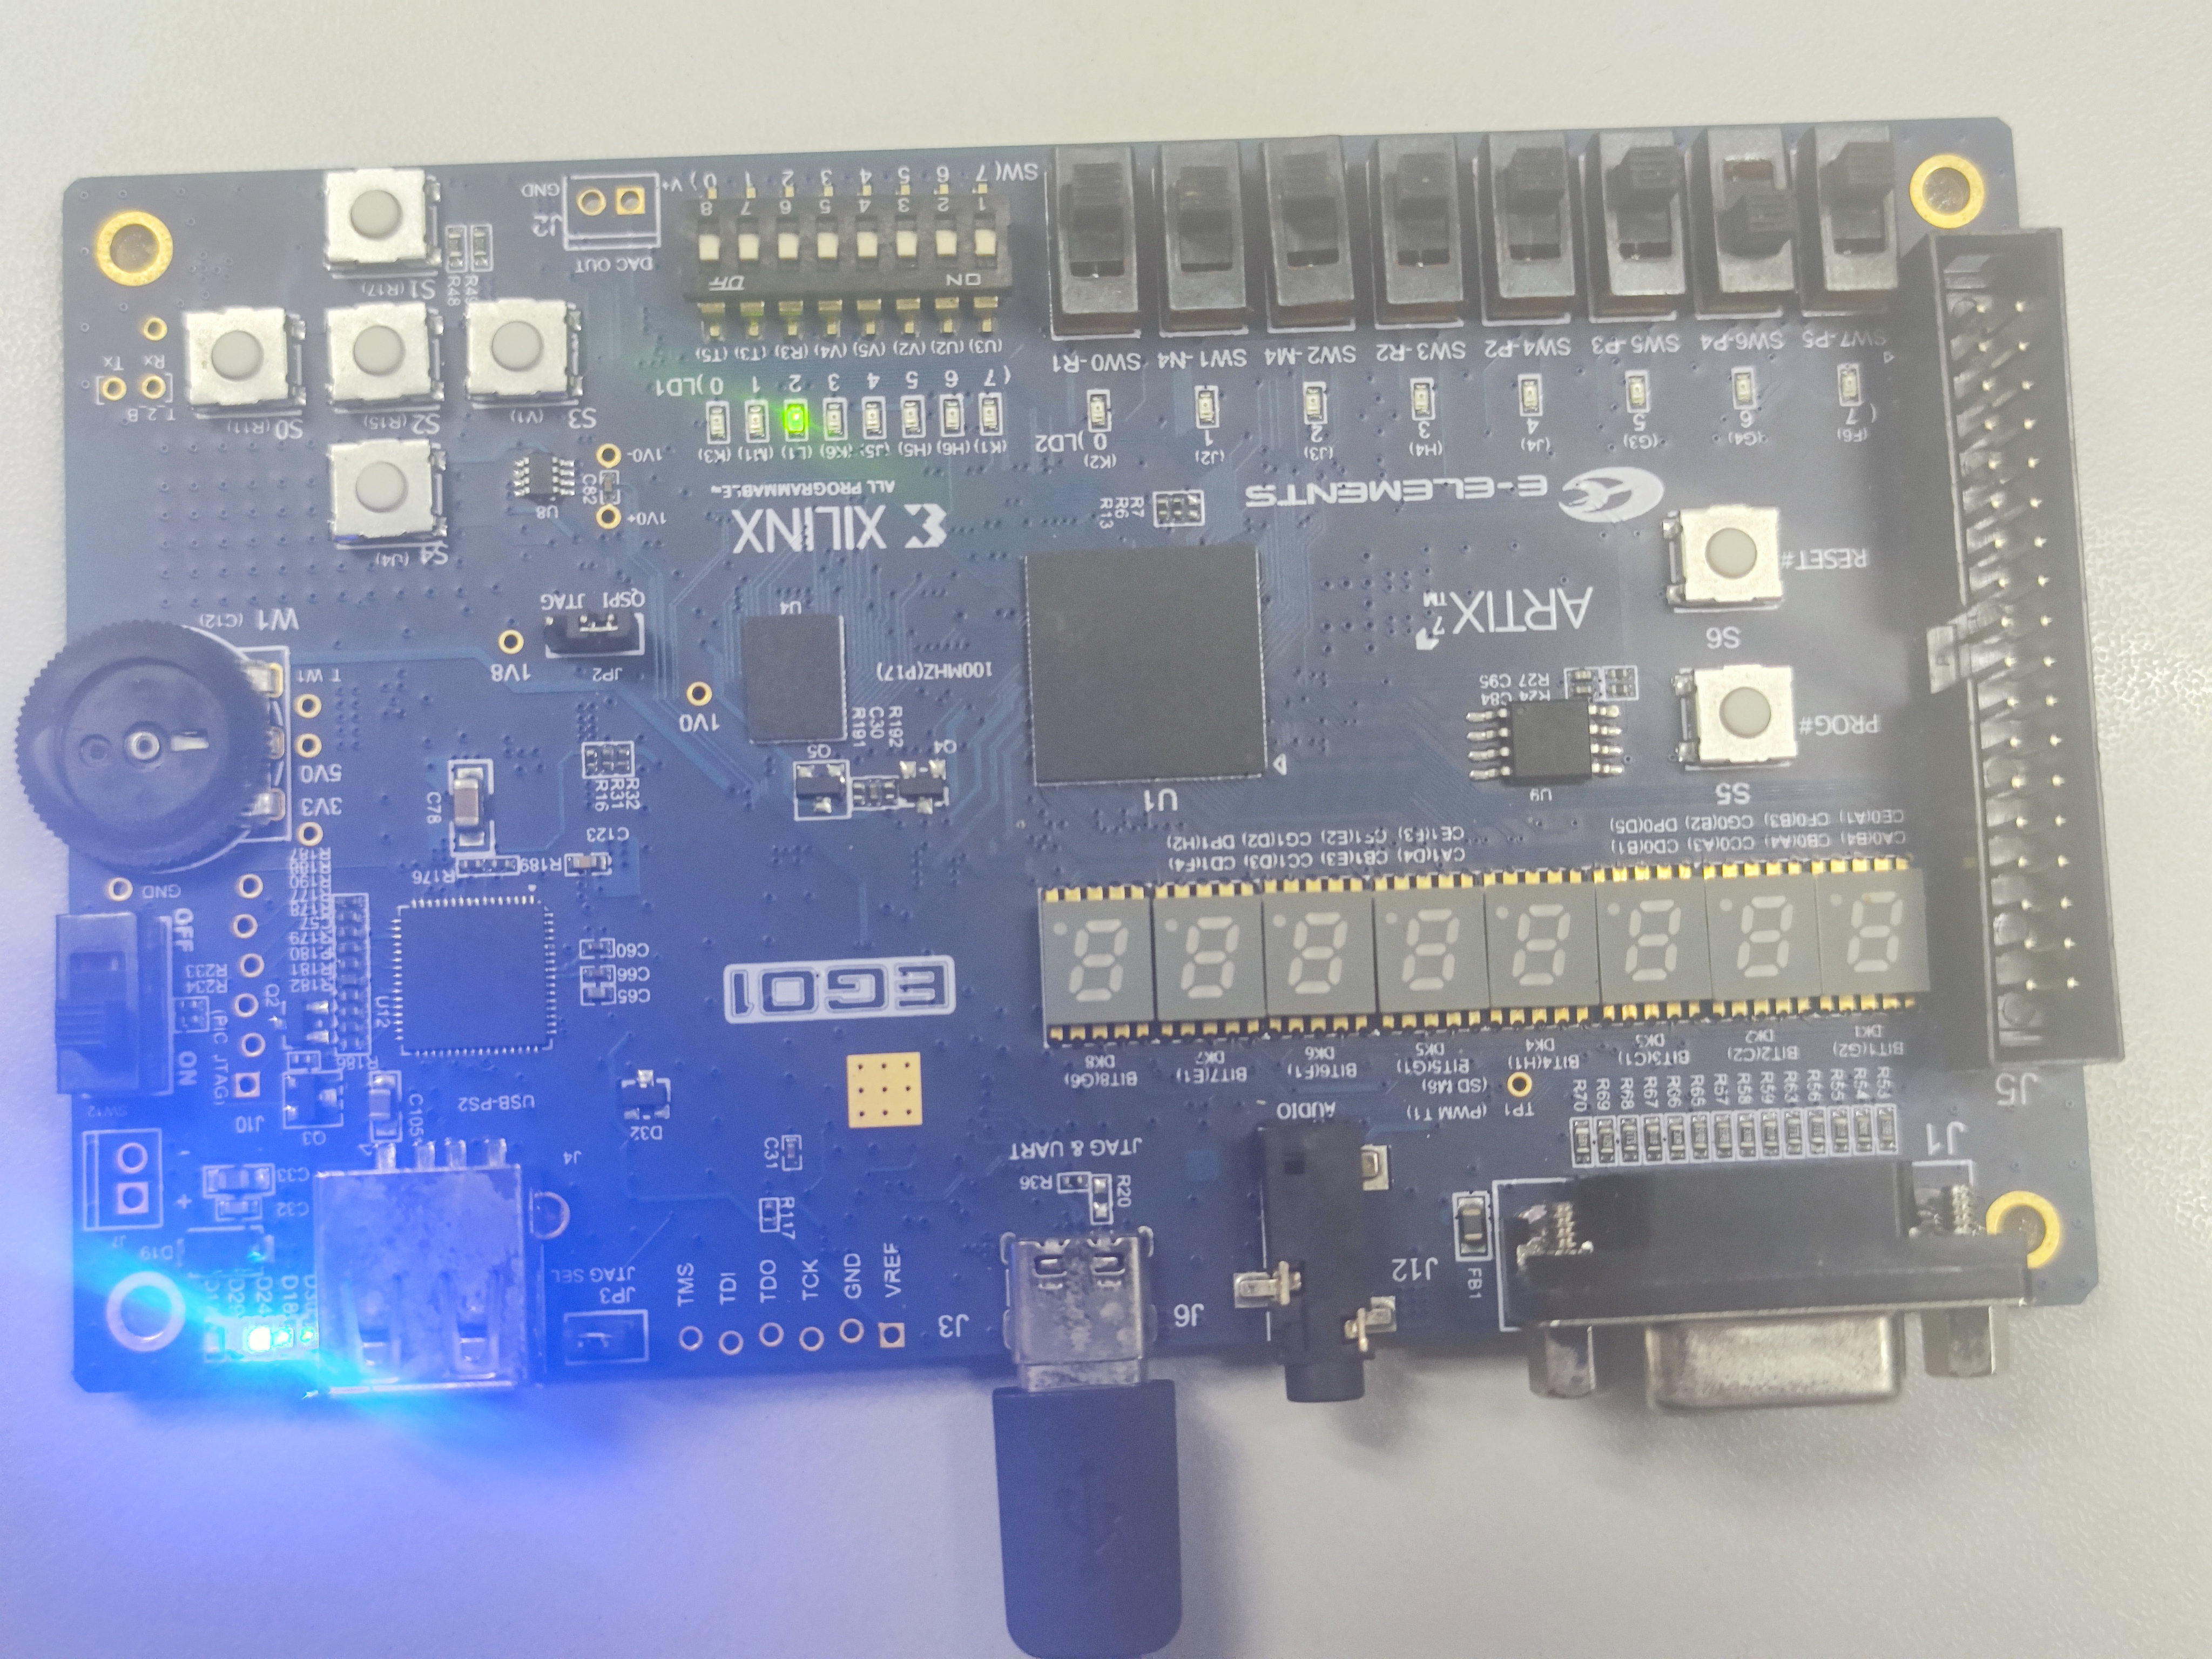
\includegraphics[width=0.5\textwidth]{流水灯1.jpg}

\end{enumerate}

通过实验,成功验证Vivado完整的开发流程,并掌握了Vivado平台、Verilog语言和开发板的使用方法。设计能够在实际硬件上正确运行,LED灯流水效果符合预期。这次实验进一步加深了我们对数字逻辑电路设计与FPGA开发流程的理解,为今后更复杂的设计和开发奠定了坚实的基础。

\subsection{基础门电路}

在实验的第二部分,我着重于使用Verilog语言在Vivado平台上实现基础的数字逻辑电路,并对其进行测试和分析。实验包括以下内容:

\begin{enumerate}
\item
  \textbf{设计文件编写}:

  \begin{itemize}
  \item
    首先,我们编写了二输入与门、六输入与门、编码器、译码器、触发器和寄存器的Verilog设计文件。这些设计文件描述了电路的逻辑功能和结构。
  \item
    在设计文件中,使用Verilog语言描述了每个电路的输入端口、输出端口和逻辑运算。
  \end{itemize}
\item
  \textbf{仿真文件编写}:

  \begin{itemize}
  \item
    接下来,我们编写了每个电路对应的仿真文件,以验证其功能正确性。
  \item
    在仿真文件中,创建仿真测试用例,并通过对仿真波形的分析来验证电路的正确性。
  \end{itemize}
\item
  \textbf{时序仿真}:

  \begin{itemize}
  \item
    对每个电路进行了时序仿真,以验证其在不同时钟周期下的运行情况。
  \item
    通过时序仿真,我们可以确定电路的响应时间和稳定性,以及是否存在时序冲突或时序问题。
  \end{itemize}
\item
  \textbf{RTL分析}:

  \begin{itemize}
  \item
    对每个电路进行了RTL分析,以检查其硬件实现是否符合预期。
  \item
    通过RTL分析,可查看逻辑综合后的电路结构,包括门级逻辑和寄存器级别的连接。
  \end{itemize}
\end{enumerate}

\paragraph{1. 二输入与门}

\begin{itemize}
\item
  电路功能:实现逻辑表达式 \(A \& B = Y \)(其中 \(A\) 和 \(B\)
  是输入,\(Y\) 是输出)
\item
  代码设计:
  
  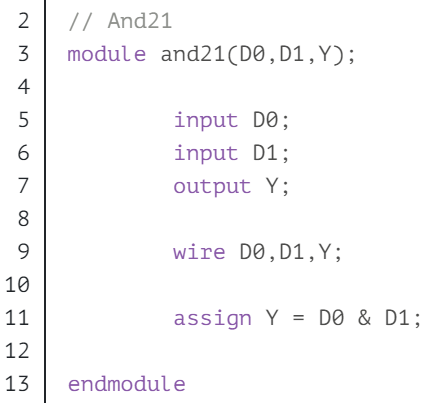
\includegraphics[width=0.4\textwidth]{AND21_Code.png}
\item
  RTL分析结果:
  
  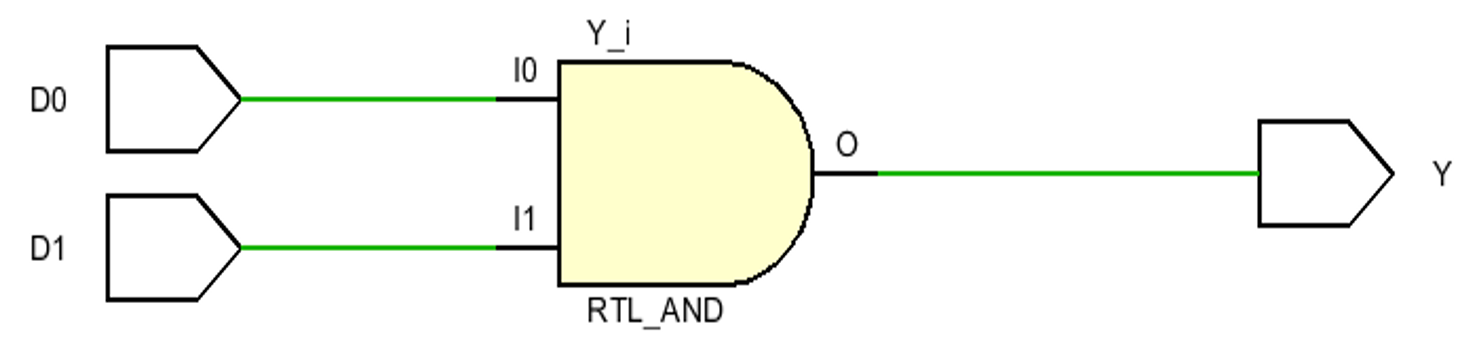
\includegraphics[width=0.5\textwidth]{AND21_RTL.png}
\item
  Simulation结果:
  
  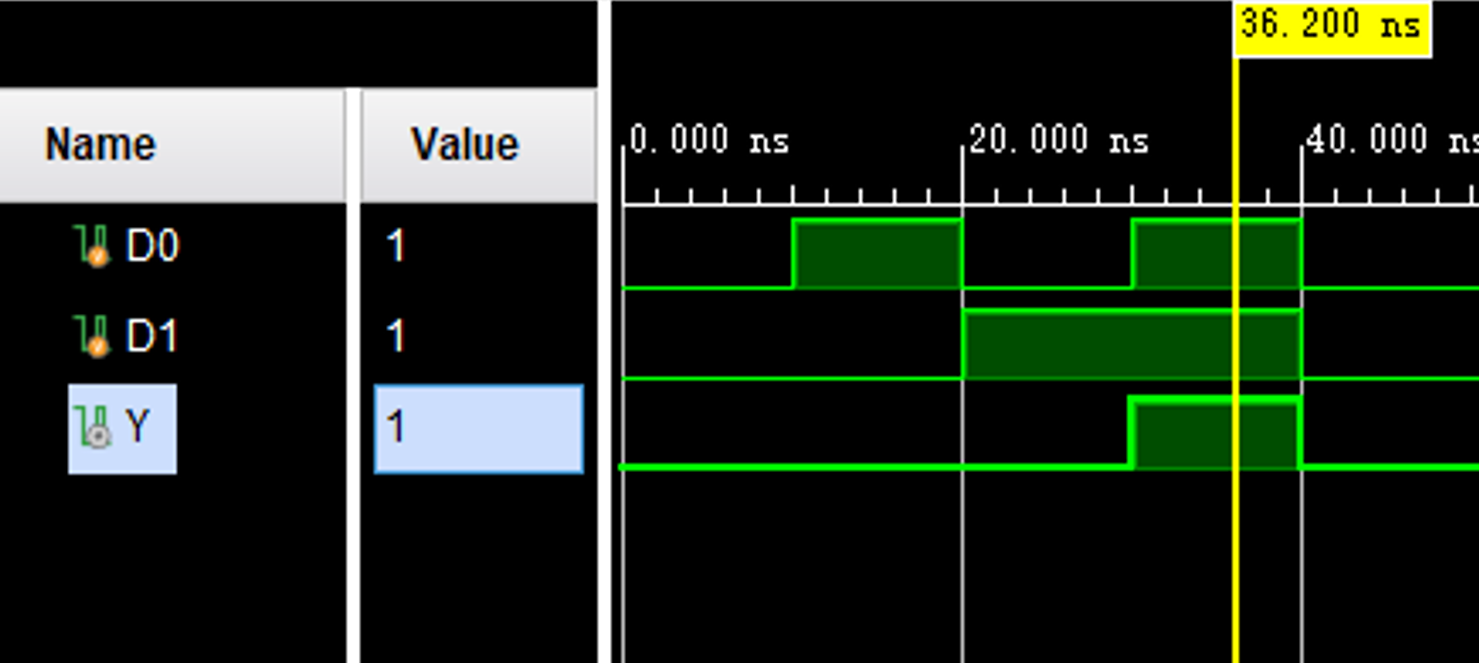
\includegraphics[width=0.5\textwidth]{AND21_Simulation.png}
\end{itemize}

\paragraph{2. 六输入与门}
\begin{itemize}
\item
  电路功能:实现逻辑表达式 \(\Pi_{i=0}^{5} A_i = Y \)(其中 \(A_i\)
  是输入,\(Y\) 是输出)
\end{itemize}

\begin{itemize}
\item
  代码设计:
  
  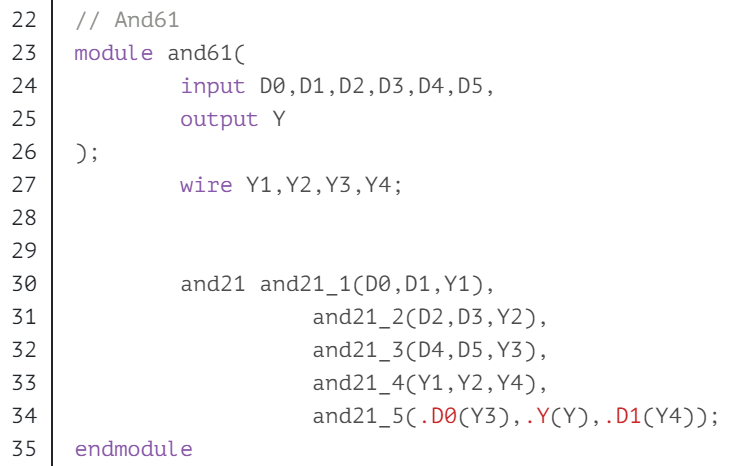
\includegraphics[width=0.4\textwidth]{AND61_Code.png}
\item
  RTL分析结果:
  
  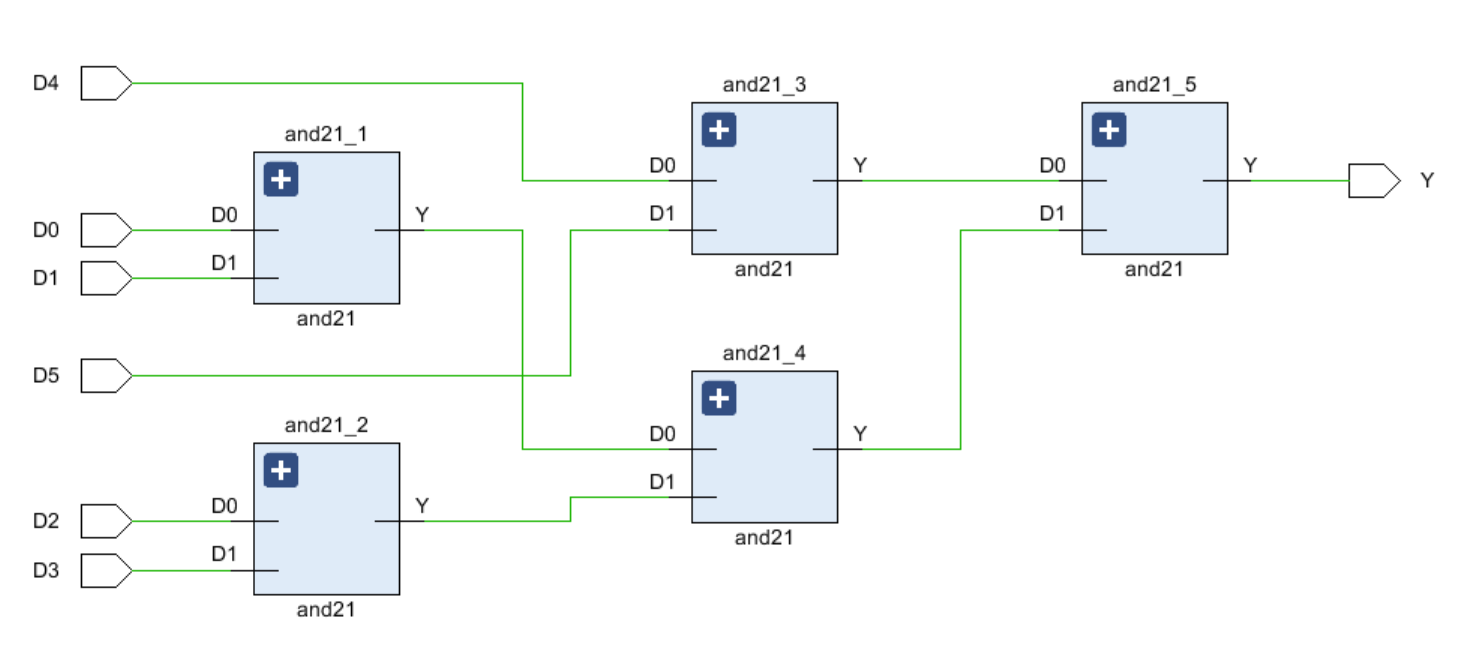
\includegraphics[width=0.5\textwidth]{AND61_RTL.png}
\item
  Simulation结果:
  
  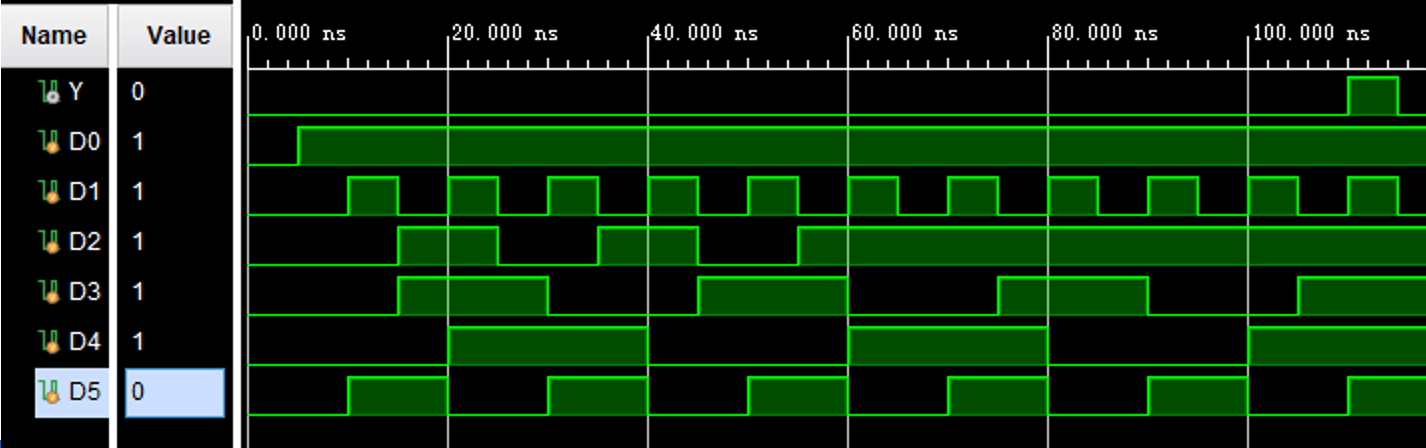
\includegraphics[width=0.5\textwidth]{AND61_Simulation.png}
\end{itemize}

\paragraph{3. 编码器}

\begin{itemize}
\item
  电路功能:实现有\(2^N\)个输入和\(N\)个输出, \(2^N\)
  位数据编码为\(N\)位数据 (\(N=3\))
\end{itemize}

\begin{itemize}
\item
  代码设计:
  
  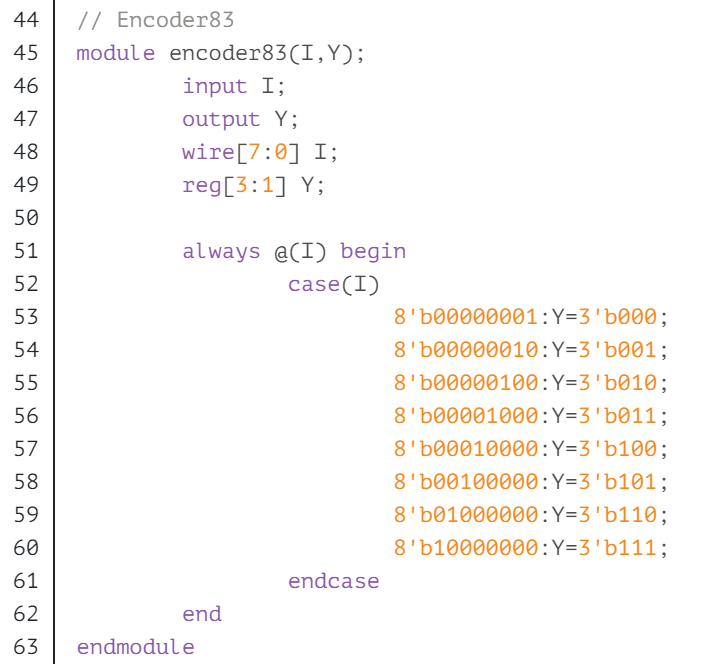
\includegraphics[width=0.4\textwidth]{ENCODER83_Code.png}
\item
  RTL分析结果:
  
  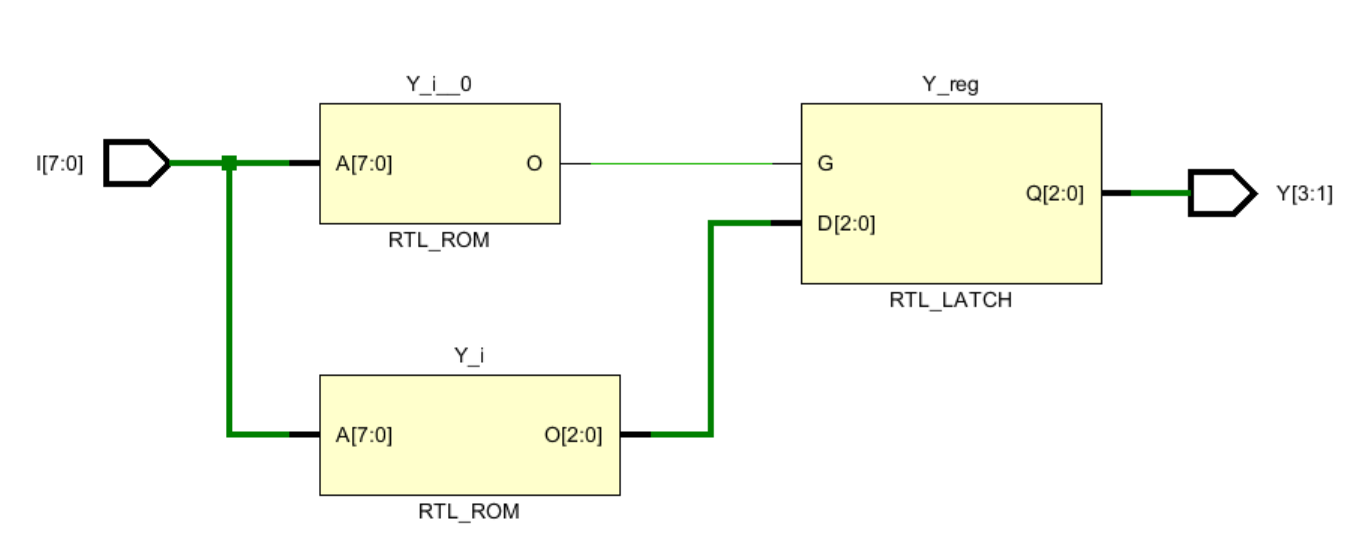
\includegraphics[width=0.5\textwidth]{ENCODER83_RTL.png}
\item
  Simulation结果:
  
  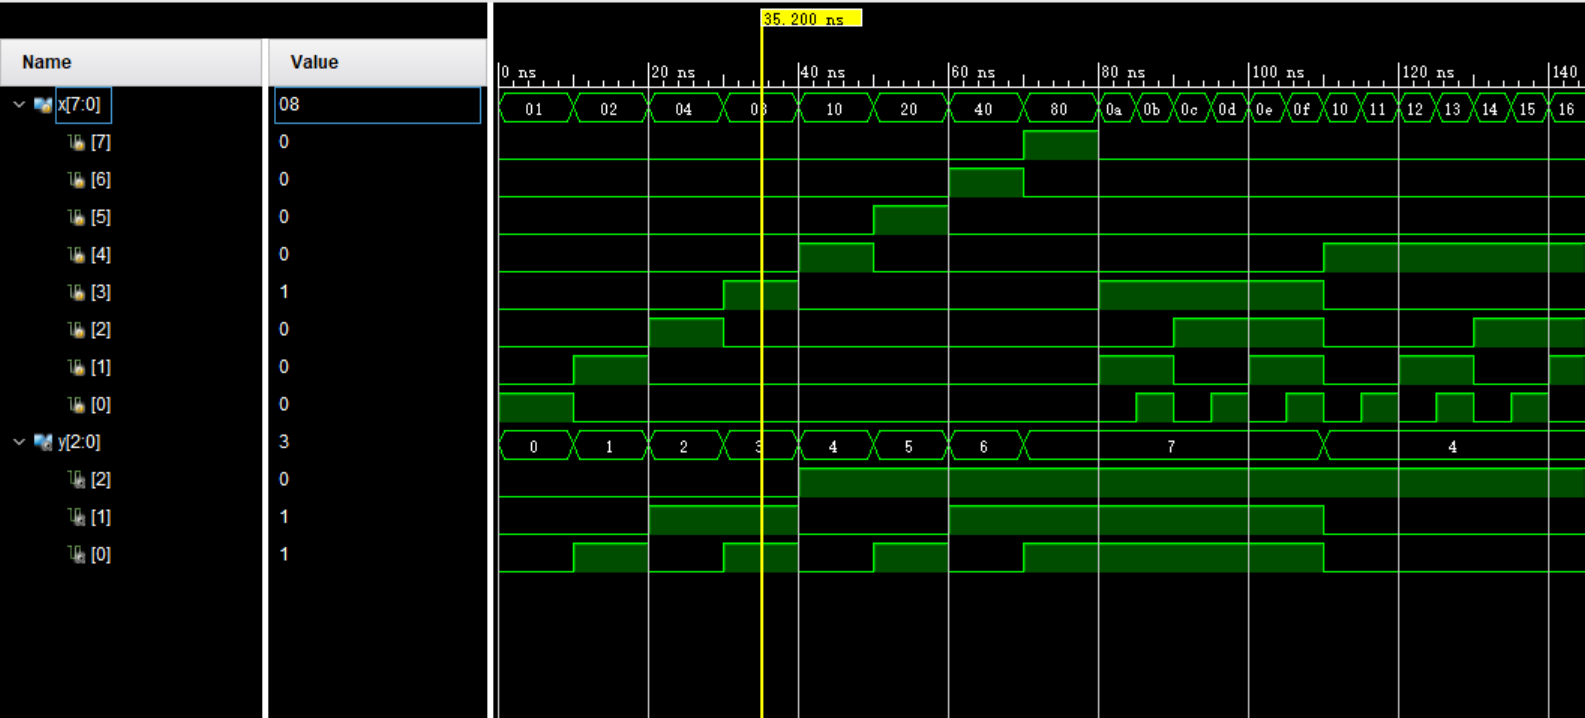
\includegraphics[width=0.5\textwidth]{ENCODER83_Simulation.png}
\end{itemize}

\paragraph{4. 译码器}

\begin{itemize}
\item
  电路功能:有\(N\)个输入和\(2^N\)个输出, 在\(2^N\)位输出中取一位有效
  (\(N=3\))
\end{itemize}

\begin{itemize}
\item
  代码设计:
  
  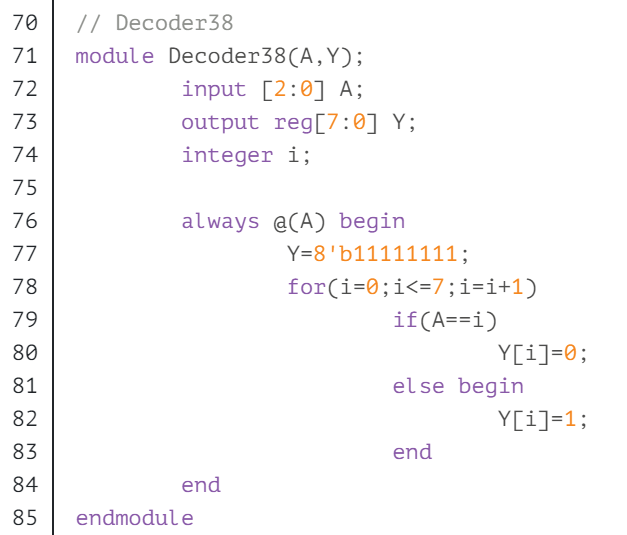
\includegraphics[width=0.4\textwidth]{DECODER_Code.png}
\item
  RTL分析结果:
  
  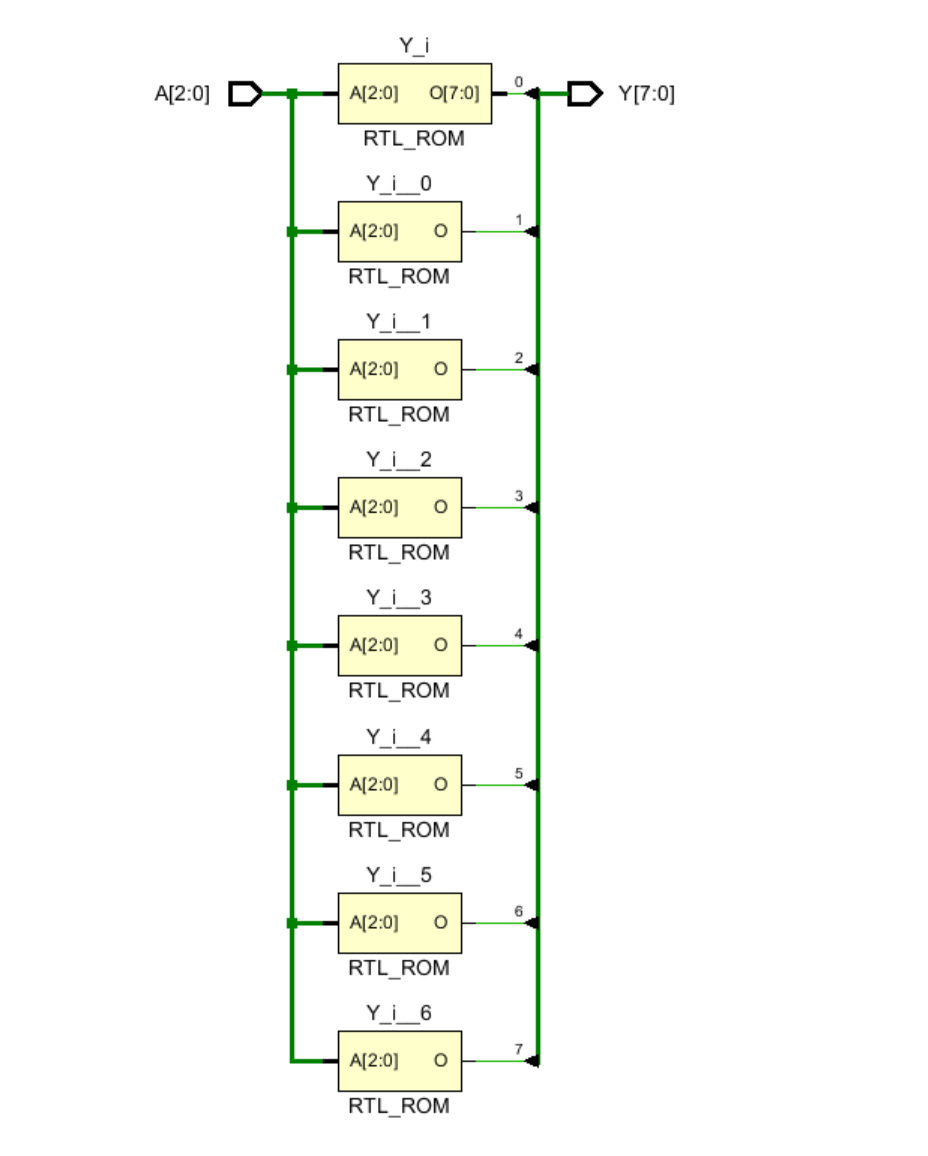
\includegraphics[width=0.5\textwidth]{DECODER_RTL.png}
\item
  Simulation结果:
  
  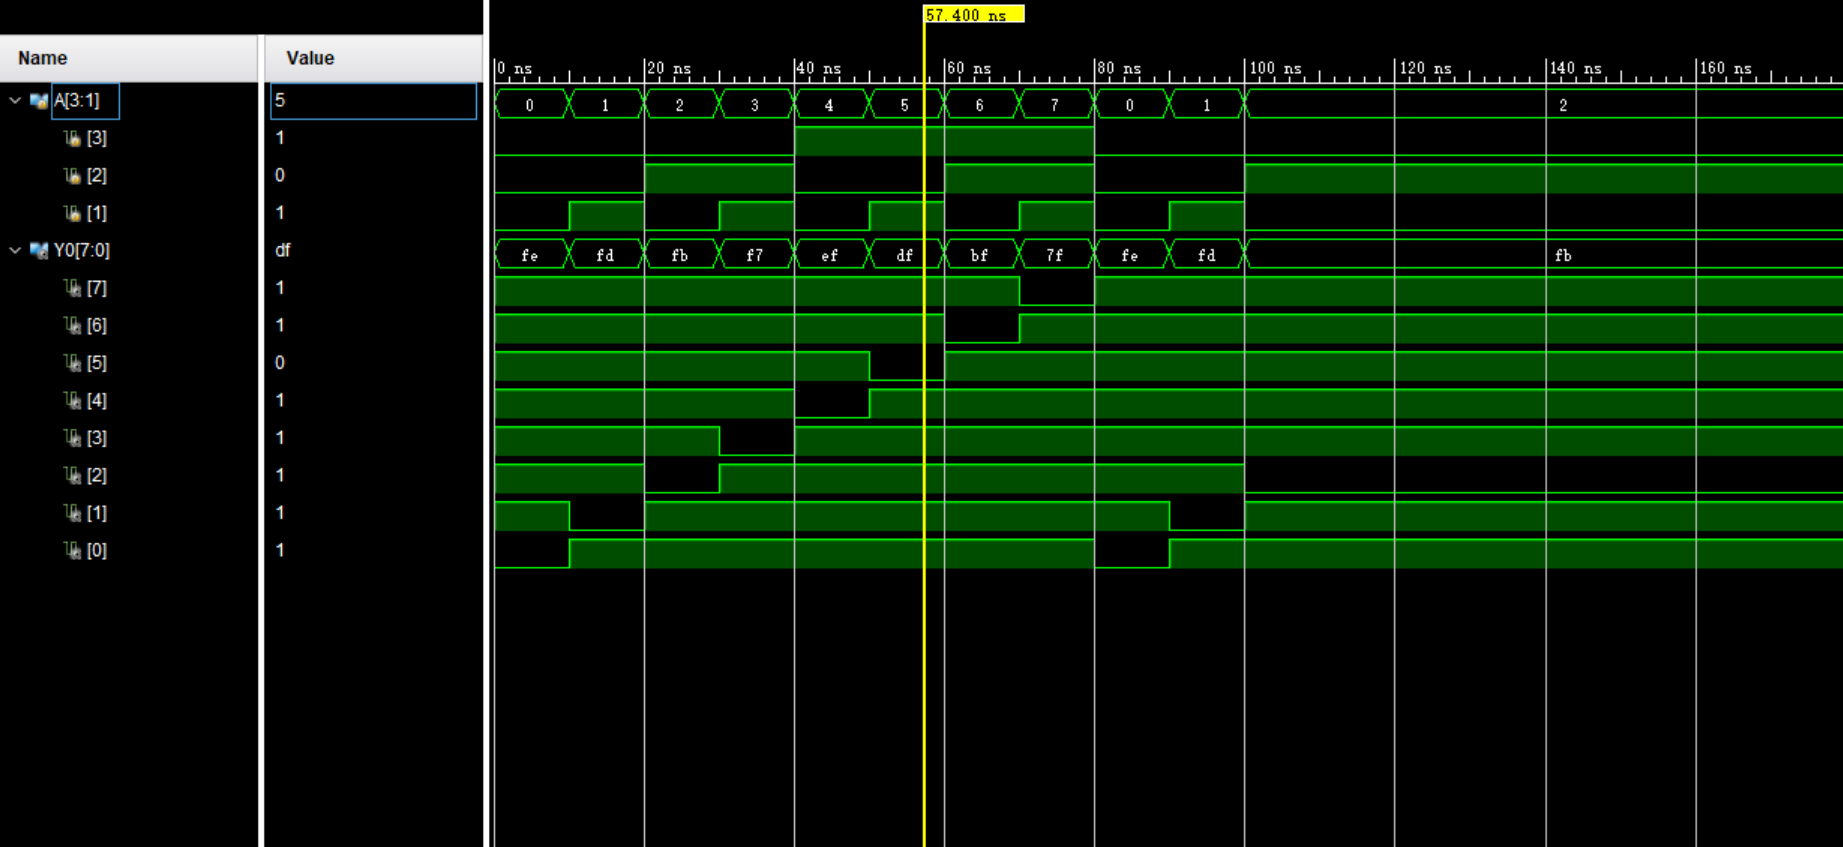
\includegraphics[width=0.5\textwidth]{DECODER_Simulation.png}
\end{itemize}

\paragraph{5. 触发器}

\begin{itemize}
\item
  电路功能:实现在时钟上升沿时,将D值复制到Q,在其他时间保持原有的状态
\end{itemize}

\begin{itemize}
\item
  代码设计:
  
  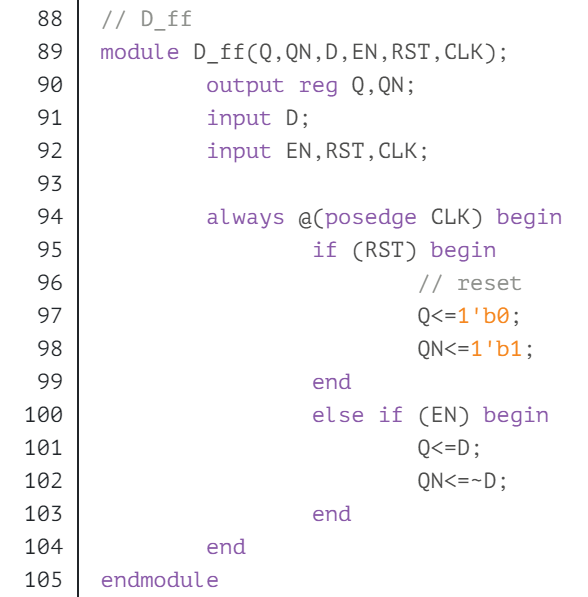
\includegraphics[width=0.4\textwidth]{DFF_Code.png}
\item
  RTL分析结果
  
  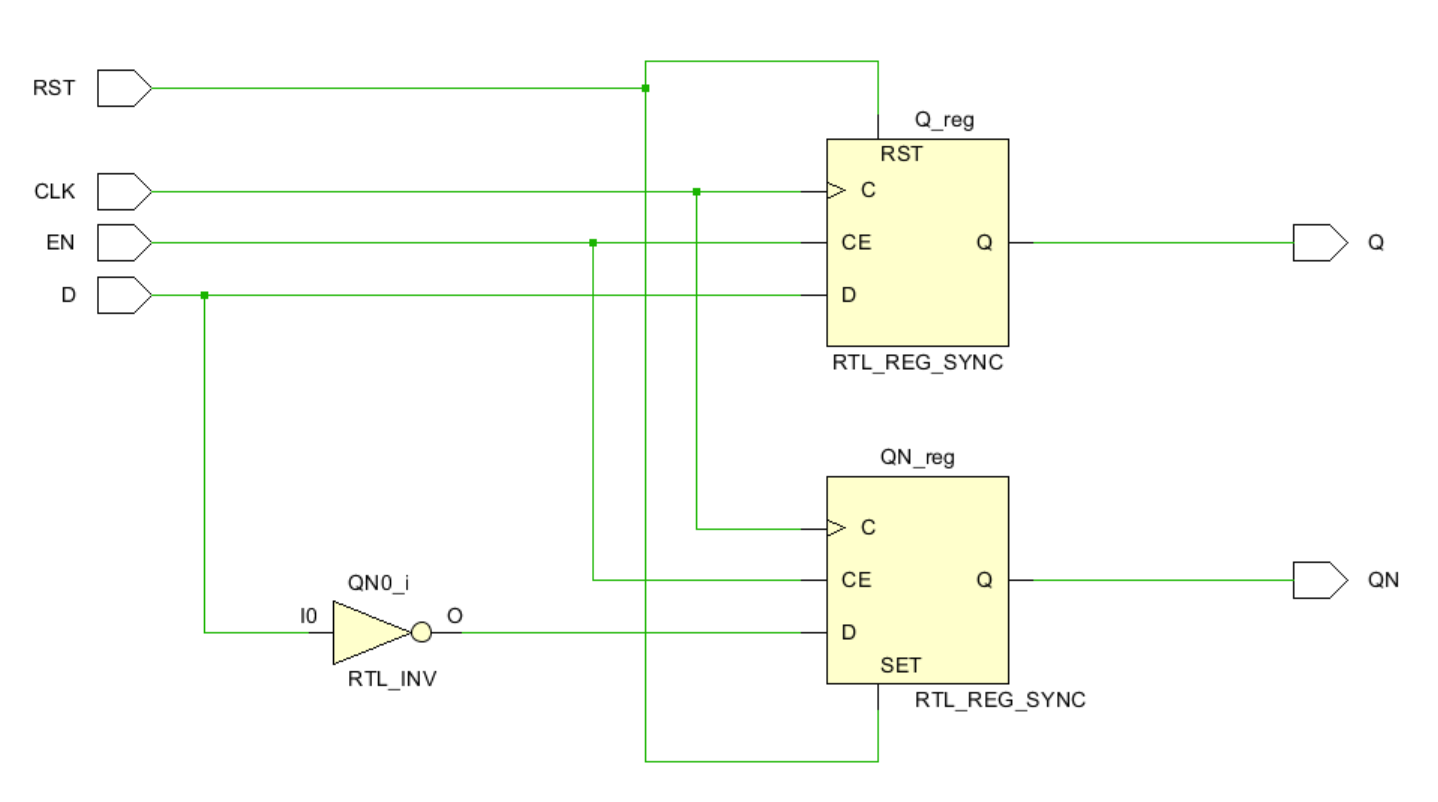
\includegraphics[width=0.5\textwidth]{DFF_RTL.png}
\item
  Simulation结果:
  
  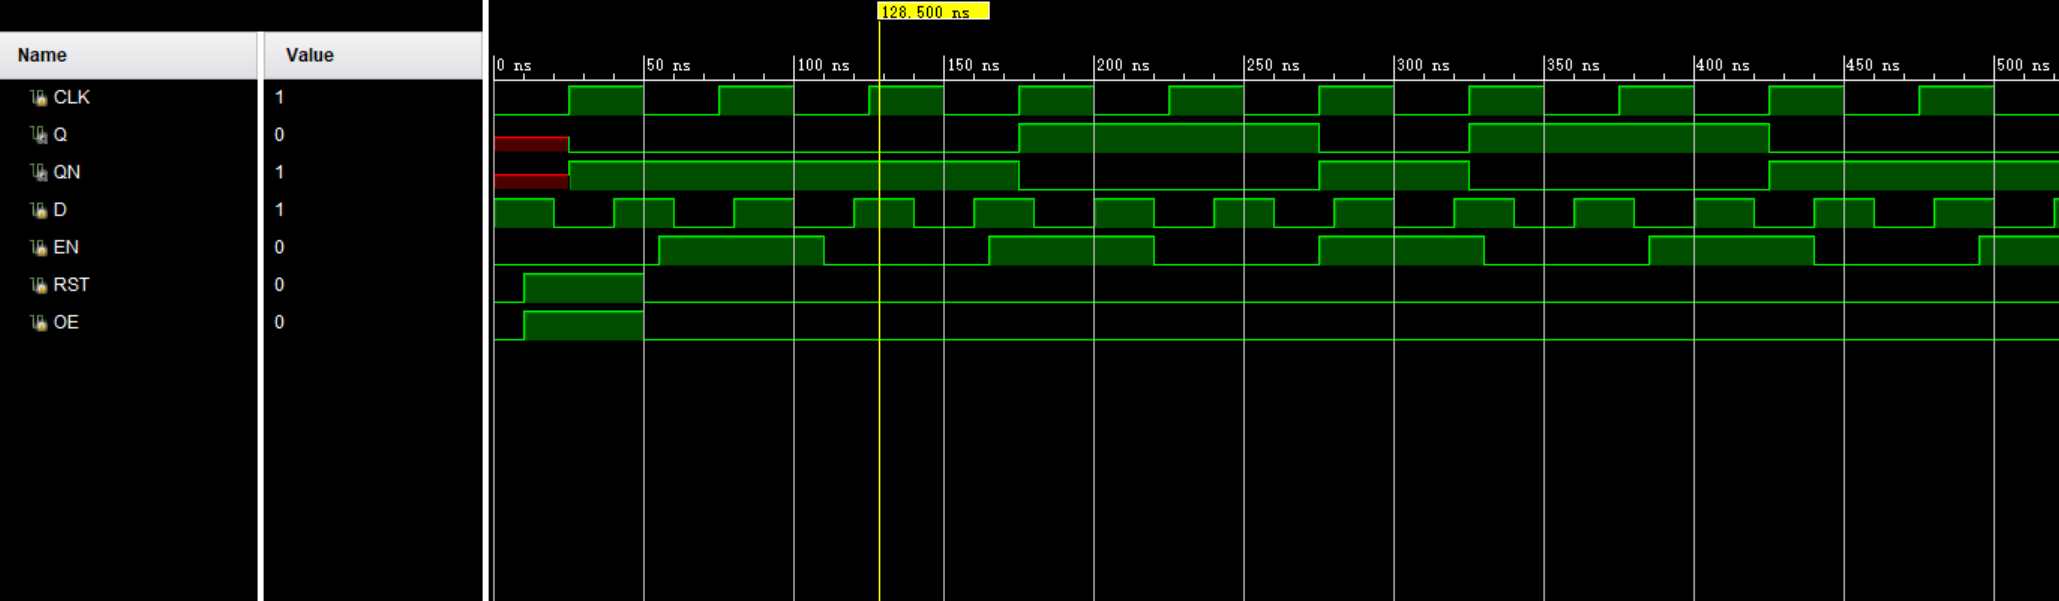
\includegraphics[width=0.5\textwidth]{DFF_Simulation.png}
\end{itemize}

\paragraph{6. 寄存器}

\begin{itemize}
\item
  电路功能:寄存器由共享同一时钟的N个触发器组成,寄存器的所有位同时被更新
\end{itemize}

\begin{itemize}
\item
  代码设计:
  
  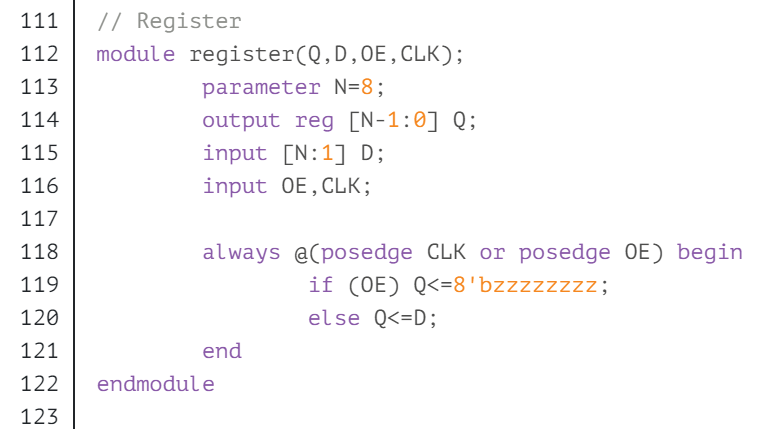
\includegraphics[width=0.4\textwidth]{REGISTER_Code.png}
\item
  RTL分析结果:
  
  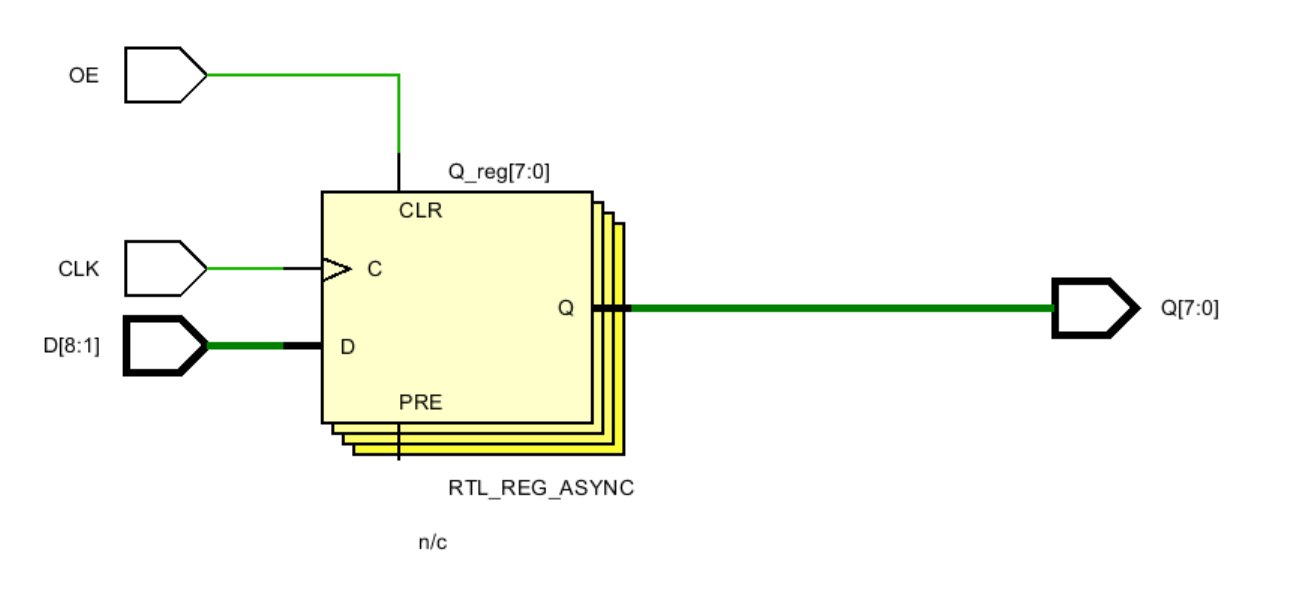
\includegraphics[width=0.5\textwidth]{REGISTER_RTL.png}
\item
  Simulation结果:
  
  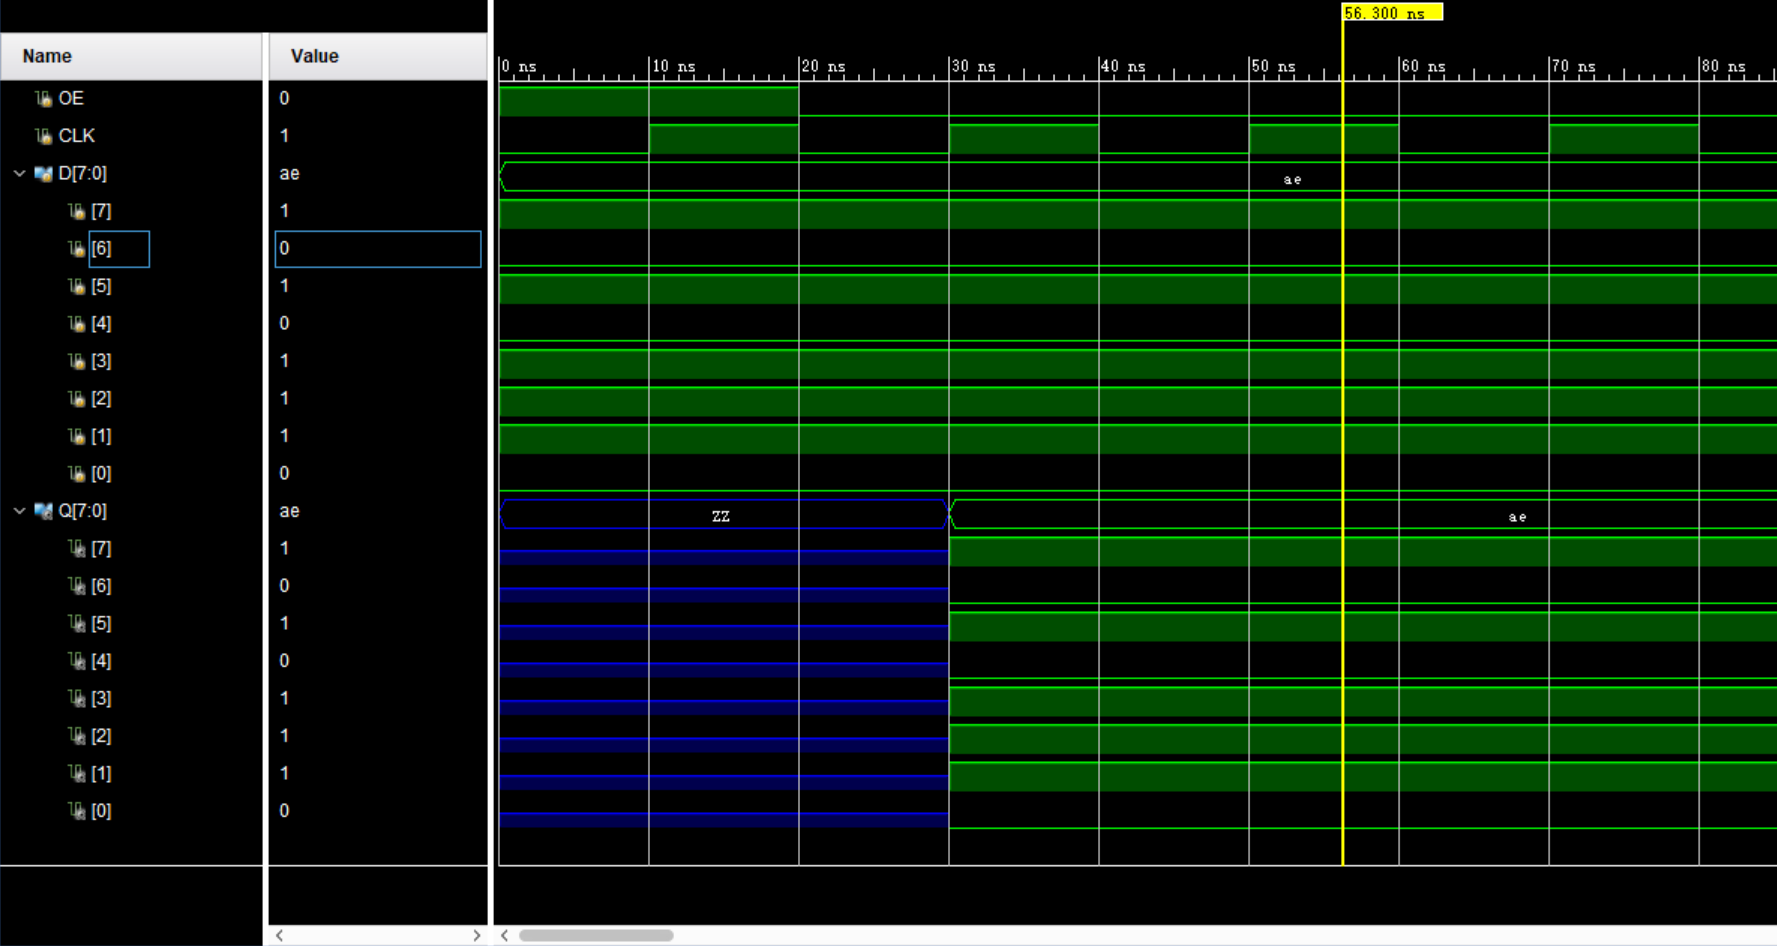
\includegraphics[width=0.5\textwidth]{REGISTER_Simulation.png}
\end{itemize}

\section{调试和心得体会}
\begin{itemize}
  \item 遇到的问题:由于第一次使用Vivado集成开发环境,对于其代码编辑环境不熟悉,导致了以下错误:
    \begin{itemize}
      \item 将0和O混淆输入
      \item 将L和1混淆输入
      \item 混淆输入全半角的分号、冒号和逗号
    \end{itemize}
  \item 调试解决过程:观察Vivado集成开发环境中对于代码语法的错误提示,即红色波浪线的位置。通过反复测试和修改代码,逐步纠正了这些初步错误,学习了代码的准确书写和语法规范。
  \item 心得体会:
    \begin{enumerate}
      \item 本次实验让我深刻理解了数字逻辑电路的设计和FPGA编程的实际应用,尤其是通过亲手编写Verilog代码和进行时序仿真,加深了我对硬件描述语言的理解。
      \item Vivado工具的使用初期相对困难,但通过不断的实践和错误修正,我学会了如何有效地利用这一强大的集成开发环境来实现复杂的电路设计。
      \item 实验过程中,我意识到细节的重要性,比如信号的命名、模块的组织和代码的可读性等,这些都对项目的成功完成至关重要。
      \item 通过分析仿真波形和RTL图,我学会了如何评估电路的性能和检测潜在的逻辑错误,这对我的调试技能有很大的帮助。
      \item 此次实验也提醒我,在面对问题和挫折时,耐心和细致的调查是解决问题的关键。
    \end{enumerate}
\end{itemize}


\end{document}
